\chapter{The Standard Model of Particle Physics}\label{ch:sm}

The Standard Model is a set of theories describing the interactions between elementary particles.
It explains three of the four known fundamental forces, namely the electromagnetic force,
the weak nuclear force, and the strong force.
It does not include  or account for gravitational interactions.

The Standard Model can be fairly characterized as the most successful theory in science.
A huge number of predictions made by the theory have been confirmed experimentally,
some to an astounding degree of accuracy.
Precision measurements of the magnetic moment of the electron have shown the experimental and theoretical values of the
fine structure constant to agree better than one part in one billion.\cite{sm-fine-structure-2008}
The ATLAS detector at the LHC has confirmed the predicted rate of particle production for a very wide range of
production processes and final states.
A summary of Standard Model measurements made by ATLAS, and their comparisons to theoretical predictions can be seen in figure~\ref{fig:sm_xsec_summary}.
The Standard Model predicted the existence of the W boson, the top quark, and the Higgs boson,
which were all later confirmed by experiment.

\begin{figure}[!ht]
    \centering
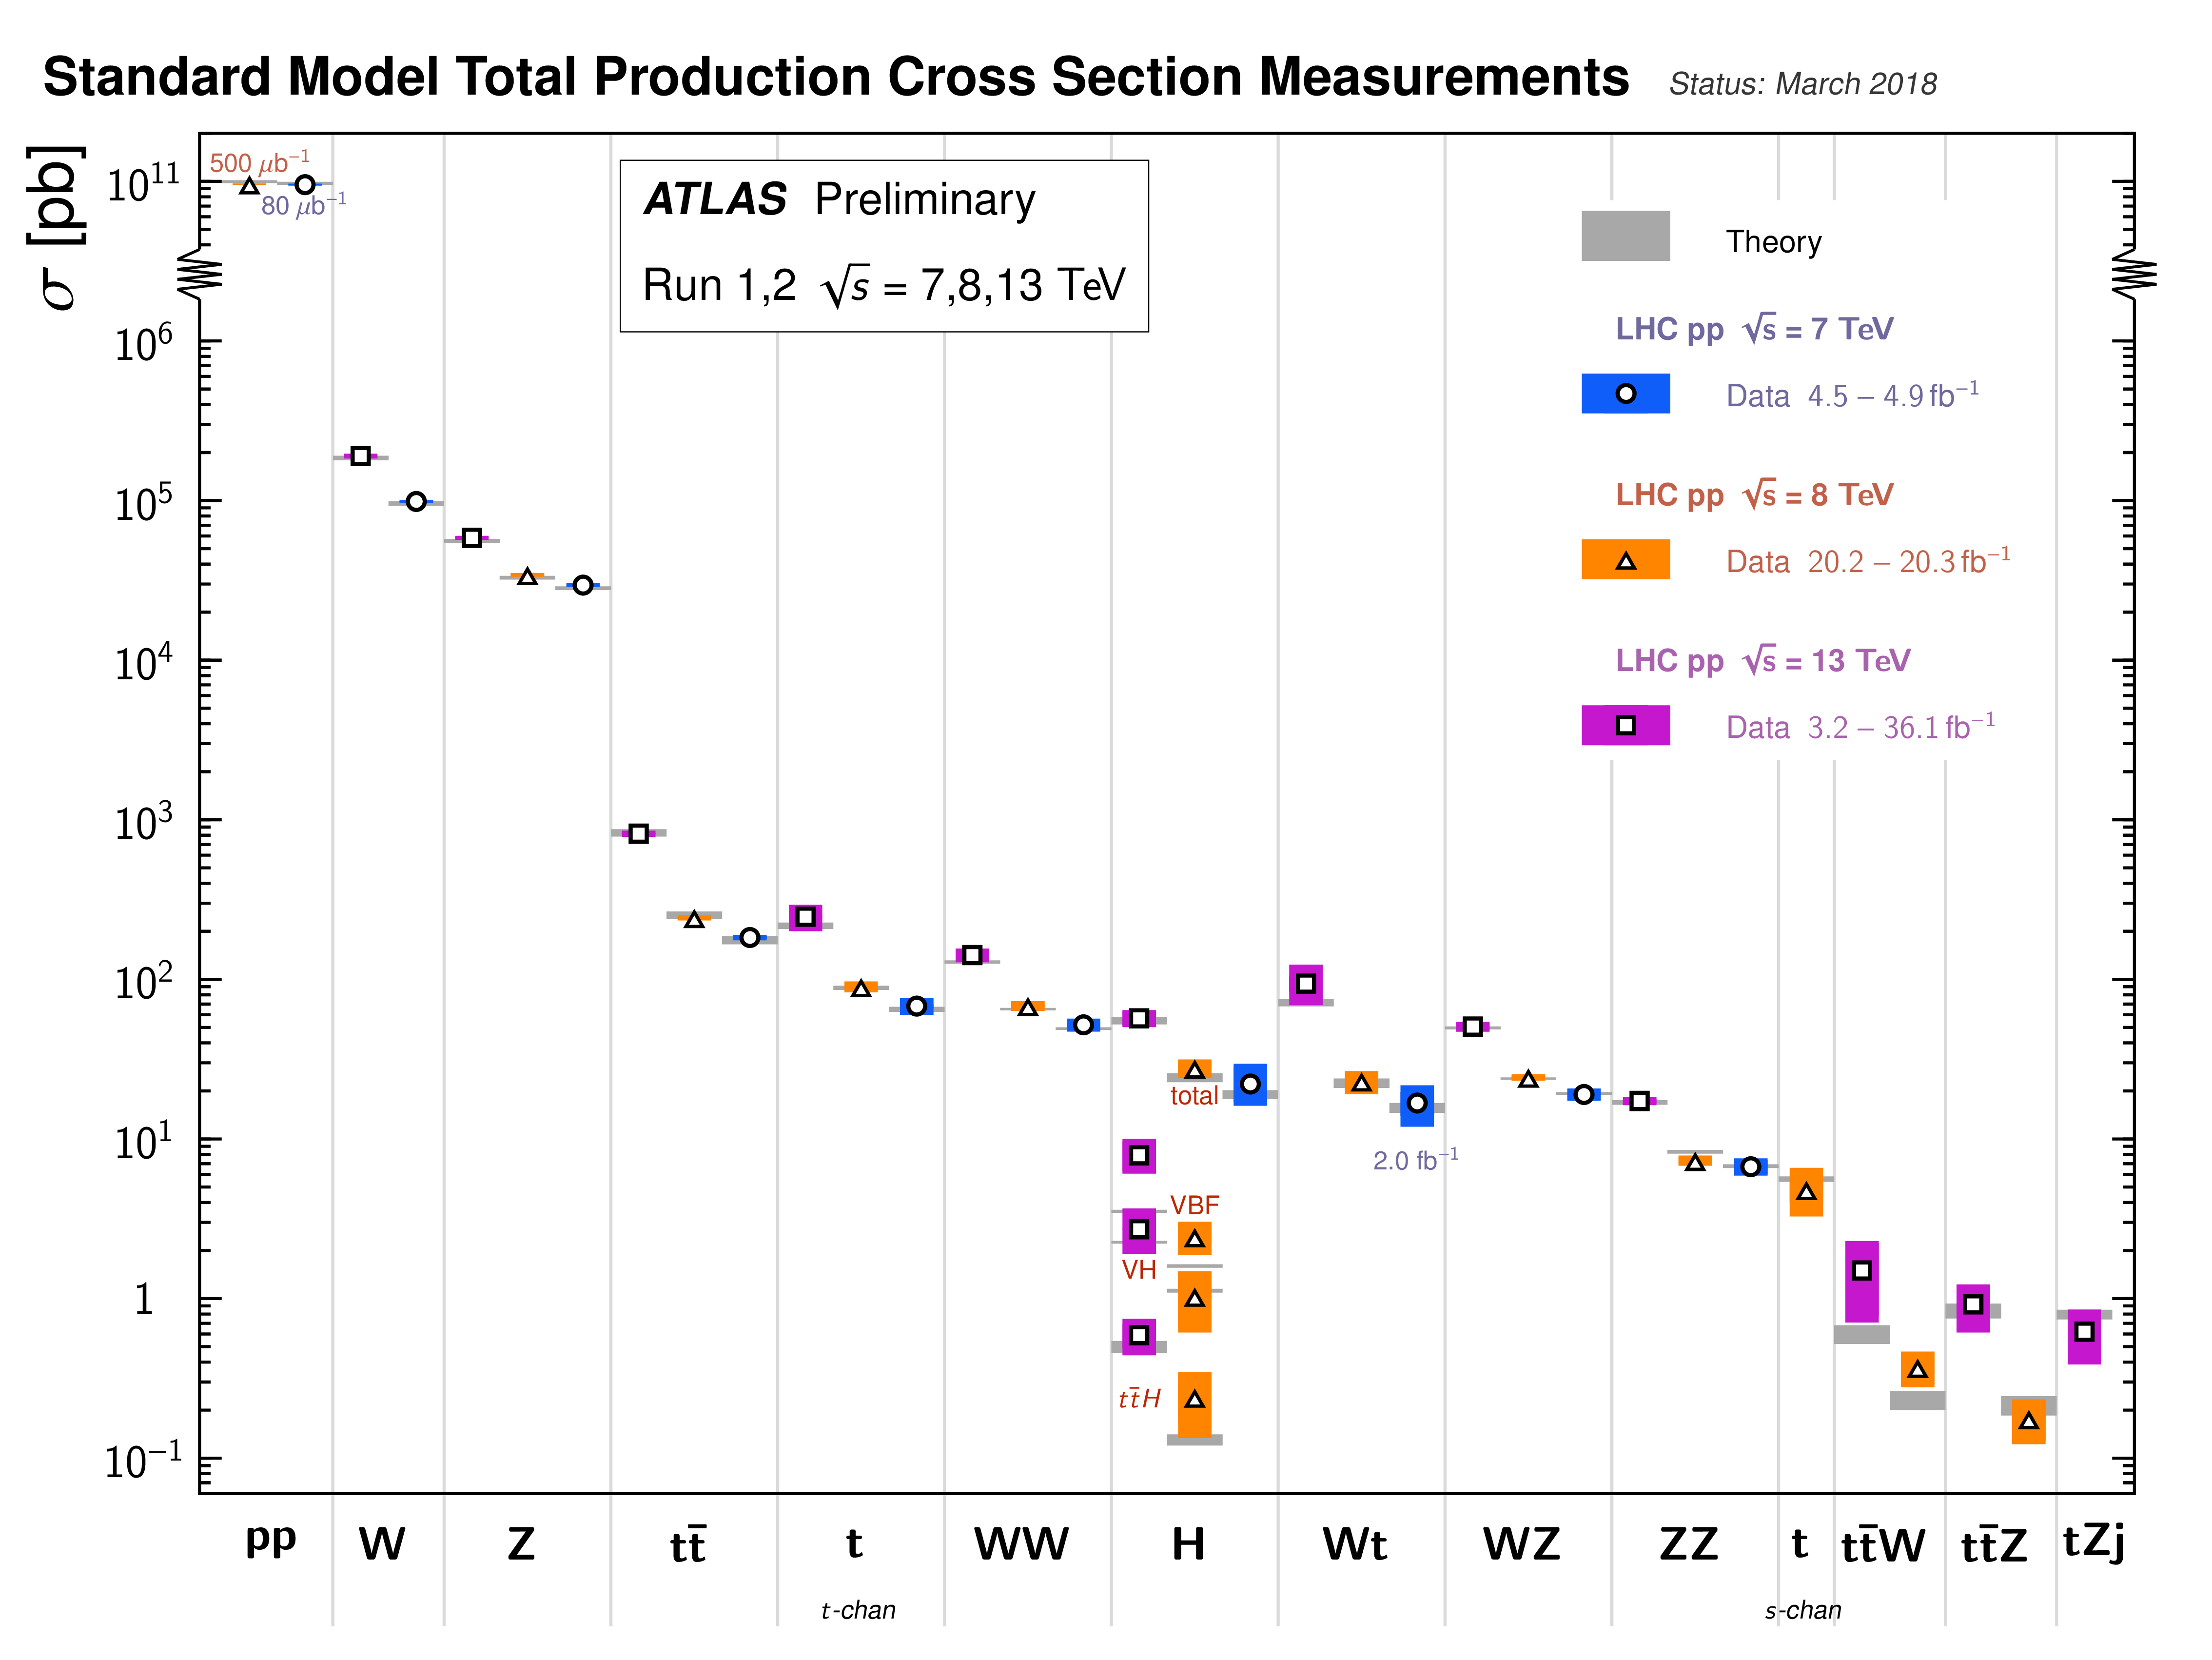
\includegraphics[width=0.6\linewidth]{sm_xsec_summary}
\caption{Summary of Standard Model production cross sections measured by ATLAS, compared to theoretical predictions.}
\label{fig:sm_xsec_summary}
\end{figure}

The Standard Model is expressed in the language of Quantum Field Theory.
The theory consists of three generations of matter fields,
specified by their representation under the gauge group $SU(3)\times SU(2)\times U(1)$ and the Poincar\'e group,
as well as a complex scalar field.
Poincar\'e symmetry consists of the Lorentz symmetry of special relativity, plus global translational symmetry.

The Standard Model is a complete theory in the sense that it is internally self-consistent,
and all particles predicted by the theory have been discovered experimentally.
However, the Standard Model does not account for all known physical phenomena,
and so cannot be considered a complete theory of nature.

\section{Electroweak Sector and the Higgs Mechanism}\label{sec:sm_ew}

\subsection{Matter fields}\label{subsec:ew_fields}

All left-handed matter fields are $SU(2)$ doublets, while their corresponding right-handed fields are $SU(2)$ singlets.
There are three generations of left-handed lepton fields:

\begin{equation}\label{eq:left_handed_leptons}
    \psi_L =
    \begin{pmatrix}
        \nu_e \\ l_e
    \end{pmatrix}_L,\;
    %
    \begin{pmatrix}
        \nu_{\mu} \\ l_{\mu}
    \end{pmatrix}_L,\;
    %
     \begin{pmatrix}
        \nu_{\tau} \\ l_{\tau}
    \end{pmatrix}_L
\end{equation}

And three generations of right-handed lepton fields:
\begin{equation}\label{eq:right_handed_leptons}
\psi_R = e_R,\; \mu_R,\; \tau_R
\end{equation}

Similarly, there are three generations each of the left-handed $SU(2)$-doublet quark fields,
each of which comes in three colors:

\begin{equation}\label{eq:left_handed_quarks}
   \psi_L =
    \begin{pmatrix}
        q_u \\ q_d
    \end{pmatrix}_L,\;
    %
    \begin{pmatrix}
        q_{c} \\ q_{s}
    \end{pmatrix}_L,\;
    %
     \begin{pmatrix}
        q_{t} \\ q_{b}
    \end{pmatrix}_L
\end{equation}

Quark color will play a role in QCD interactions, as discussed in the next section.
There are also the corresponding $SU(2)$-singlet right-handed fields:

\begin{equation}\label{eq:right_handed_quarks}
\psi_R = q_{uR},\; q_{dR},\; q_{cR},\; q_{sR},\; q_{tR},\; q_{bR}
\end{equation}

\subsection{Symmetries and Lagrangian}\label{subsec:ew_lagrangian}
The symmetry constraining the electroweak sector of the Standard Model Lagrangian is $SU(2)_L \times U(1)_Y$.
The subscript $L$ for the $SU(2)$ group indicates that it only acts on the left-handed fields in the theory.
As we've seen, right-handed fields appear as $SU(2)$ singlets.
The Lagrangian density satisfying the required symmetries, including all renormalizable terms, is:

\begin{equation}\label{eq:ew_lagrangian}
    \mathcal{L}_{EW} = \mathcal{L}_{kin} + \mathcal{L}_{\text{interactions}}
\end{equation}

The kinetic part of the electroweak Lagrangian is:

\begin{equation}\label{eq:ew_kin}
    \mathcal{L}_{kin} = -\frac{1}{4}W^{\mu \nu}_{a}W_{\mu \nu}^{a}-\frac{1}{4}B^{\mu \nu}B_{\mu \nu}
\end{equation}

Where $W_\mu^a$ are the three $SU(2)_L$ gauge bosons, $B_\mu$ is the $U(1)_Y$ (hypercharge) gauge boson,
and $W_\mu\nu = \partial_{\mu} W_{\nu} - \partial_{\nu} W_{\mu}$.

The part of the electroweak Lagrangian describing electroweak interactions is:

\begin{equation}\label{eq:ew_int}
    \mathcal{L}_{\text{interactions}} = \sum_{\text{generations}}\left[\frac{g}{2}\bar{\psi}_{L}\gamma^\mu\sigma^i W_\mu^i \psi_L+
    g'B_\mu\left(Y_{\psi_L}\bar{\psi}_L\gamma^\mu\psi_L + Y_{\psi_R}\bar{\psi}_R\gamma^\mu \psi_R\right)\right]
\end{equation}

Where $\gamma^\mu$ are the Dirac gamma matrices, Y is the hypercharge associated with the relevant field.
Left-handed leptons and quarks have weak hypercharge $Y = -1$ and $Y = 1/3$, respectively.
Right-handed leptons have weak hypercharge $Y = -2$, while right-handed up-type quarks have weak hypercharge $Y = 4/3$,
and right-handed down-type quarks have weak hypercharge $Y = -2/3$.

This Lagrangian describes the charged-current and neutral-current weak interactions, as well as weak gauge boson self-interactions.
However, it is insufficient to describe nature because the gauge bosons are massless in this theory.
It would be impossible to include gauge boson mass terms in the electroweak Lagrangian without explicitly breaking the symmetry.
Similarly, it's impossible to introduce Lorentz-invariant fermion mass terms that keep the Lagrangian invariant under $SU(2)_L \times U(1)_Y$.
In order to reconcile this theory with the experimentally observed fact of massive weak gauge bosons and massive fermions,
an entirely new field will have to be introduced.

\subsection{Spontaneous symmetry breaking}\label{subsec:ew_higgs}

The original $SU(2)_{L}\times U(1)_Y$ symmetry will be spontaneously broken, via the nonzero Higgs vacuum expectation value, to $U(1)_{QED}$.
This process of spontaneous symmetry breaking (SSB) generates fermion masses, electroweak gauge boson masses,
and the Yukawa coupling terms between fermions.
It also generates a new massive real scalar field, known as the Higgs field.

We introduce a new $SU(2)$-doublet complex scalar field, $\phi$, as well as a potential of the form:

\begin{equation}\label{eq:higgs_potential}
    V(\phi) = \mu^2 \phi^\dagger\phi + \lambda(\phi^\dagger\phi)^2
\end{equation}

With $\lambda > 0$ and $\mu^2 <0$.
The minimum energy state satisfies: $\phi^\dagger\phi = \frac{-\mu^2}{2\lambda}$.

We can then re-parameterize the scalar field as:

\begin{equation}\label{eq:higgs_param}
    \phi = \exp{\left(i\frac{\sigma_i}{2}\theta^i(x)\right)}\frac{1}{\sqrt{2}}\begin{pmatrix} 0 \\ v+H(x) \end{pmatrix}
\end{equation}

Where $H(x)$ and $\theta^i(x)$ are real-valued fields,
and $v = \sqrt{\frac{-\mu^2}{\lambda}}$ is the vacuum expectation value of the Higgs field.

Because of the $SU(2)_L$ symmetry of the theory, we are free to choose convenient values for $\theta_i(x)$,
without affecting the outcome of any observable predictions.
Selecting $\theta_i(x) = 0$, the additional kinetic term required in the Lagrangian is:

\begin{equation}\label{eq:higgs_kinetic}
    \Delta\mathcal{L}_{EW} = \left(D_{\mu}\phi\right)^{\dagger}\left(D_{\mu}\phi\right)
    =\frac{1}{2}\partial_{\mu}H \partial^{\mu}H + (v+H)^{2}\left(\frac{g^2}{4}W_\mu^\dagger W^\mu
    + \frac{g^2}{8\cos^2 {\theta_W}}Z_\mu Z^\mu\right)
\end{equation}

Where $W_\mu$ and $Z_\mu$ are mass eigenstates of the electroweak gauge fields,
linear combinations of the original $W_\mu^a$ and $B_\mu$.

This has added interaction terms between the Higgs field and the $W$ and $Z$ bosons,
as well as quadratic terms for these same bosons.
A quadratic term in the Lagrangian is physically the same as having a mass term in the Lagrangian.

So we find that the $W$ and $Z$ boson masses are:

\begin{equation}\label{eq:wz_masses}
    M_w = \frac{1}{2}vg,\; M_Z = \frac{M_W}{\cos{\theta_W}}
\end{equation}

Through SSB, electroweak gauge boson masses have been generated without requiring explicit mass terms in the Lagrangian.

The introduction of this scalar field and its associated potential also generates fermionic mass terms,
couplings between the fermions and the scalar field, and a mass term for the scalar field itself.

Like with the gauge bosons, adding an explicit fermionic mass term would break the $SU(2)_L \times U(1)_Y$ symmetry of the theory.
However, the introduction of the new scalar field allows for additional terms in the Lagrangian,
which can be written, in unitary gauge, as:

\begin{equation}\label{ew:yukawa_lagrangian}
    L_Y = \frac{1}{\sqrt{2}}\left(v+H\right)\left(c_{1}\bar{d}d+c_2\bar{u}u+c_3\bar{e}e\right)
\end{equation}

Once again, after spontaneous symmetry breaking, there appear terms in the Lagrangian that are quadratic in the fields.
These are mass terms for the fermions, and like for the gauge bosons, the masses are proportional to the Higgs vacuum
expectation value.

\begin{equation}\label{ew:fermion_masses}
    m_d = -c_1\frac{v}{\sqrt{2}},\; m_u = -c_2\frac{v}{\sqrt{2}},\; m_e = -c_3\frac{v}{\sqrt{2}}
\end{equation}

Unlike for the gauge bosons, we find no testable relationship between the fermion masses,
since the coefficients are all free parameters of the theory.

The Higgs mechanism allows for the generation of masses for electroweak gauge bosons and for fermions without explicitly
breaking the original symmetry of the theory.
Additional consequences arising from the Higgs mechanism are the relationship between $Z$ and $W$ boson masses,
the existence of a new massive scalar field, and interactions between this field and the fermions and gauge bosons.
The massive particle associated with this field, the Higgs boson, was discovered in 2012 by the ATLAS and CMS collaborations.

\section{Quantum Chromodynamics}\label{sec:sm_qcd}

Quantum Chromodynamics (QCD) is the part of the Standard Model concerned with strong interactions.
Because protons are bound states of quarks and gluons,
QCD is needed for making any calculation of event rates at a proton-proton collider.
It's particularly important for understanding the behavior of jets, which will be described in detail in chapter~\ref{ch:jets}.
The particular structure of the theory yields very different behavior at high energy and low energy.
At high energy, where the coupling strength is low, quarks and gluons are only weakly bound,
so the theory behaves as an approximately free theory, a property known as asymptotic freedom.
At lower energies, the coupling strength grows, and quarks and gluons become strongly bound,
a property known as confinement.

\subsection{Matter fields}\label{subsec:matter fields}

The fields involved are the quark fields, which also participate in electroweak interactions.
In the case of QCD, the quarks are in the fundamental $\boldsymbol{3}$ representation of $SU(3)$:

\begin{equation}\label{eq:qcd_fields}
    \psi = \begin{pmatrix}\psi_R \\ \psi_G \\ \psi_B \end{pmatrix}
\end{equation}

Where $R,\;G,\;B$ stand for the red, green, and blue color charges.
The theory will be invariant under local transformations of this color space.

\subsection{Symmetries and Lagrangian}\label{subsec:qcd_lagrangian}

Like the electroweak theory, QCD is a non-Abelian gauge theory.
The Lagrangian is generated by positing the transformations under which the Lagrangian is invariant,
and including all terms that respect these symmetries.
For QCD, the symmetry group is $SU(3)$, yielding the following Lagrangian:

\begin{equation}\label{eq:qcd_lagrangian}
    \mathcal{L}_{QCD} = \sum_{generations}i\bar{\psi}D_\mu\gamma^\mu\psi-\frac{1}{4}G_{\mu\nu}^a G_a^{\mu\nu}
\end{equation}

Where

\begin{equation}\label{eq:qcd_deriv}
D_\mu = \partial_\mu - i g_s G_\mu^a T^a
\end{equation}

is the gauge-covariant derivative, $g_s$ is the strong coupling constant, $G_\mu^a$ are the eight gluon fields,
and $T^a$ are the infinitesimal generators of $SU(3)$.
The gluon field strength tensor, $G_{\mu\nu}^a$, is defined as:

\begin{equation}\label{eq:qcd_field_strength}
    G_{\mu\nu}^a = \partial_\mu G_\nu^a - g_s f^{abc} G_\mu^b G_\nu ^c
\end{equation}

Where $f^{abc}$ are the $SU(3)$ structure constants.
This Lagrangian describes the kinematics of massless quarks, their interactions with gluons, and gluon self-interactions.
Quarks are given mass through electroweak symmetry breaking, as described in~\ref{subsec:ew_higgs}.

\subsection{QCD coupling constant}\label{subsec:qcd_coupling}

A consequence of the gluon self-interaction in the QCD Lagrangian is that the value of the strong coupling constant,
$g_s$, depends on the energy scale.
The rate of change of the coupling as energy increases is governed by the $\beta$ function,

\begin{equation}\label{eq:sm_qcd_beta}
    \beta\left(\alpha_s\right) = \frac{\alpha_s}{2\pi}\left(\frac{11}{3}n_{\text{colors}}-\frac{4}{3}n_{\text{flavors}}\right)
\end{equation}

Where $\alpha_s = g_s^2 / 4\pi$.
In QCD, there are three colors and three flavors, the consequence of which is that the coupling constant descreases with energy.
This is known as the "running" of the coupling constant, and results in very different predictions for the theory at different energy scales.
Figure~\ref{fig:sm_qcd_coupling} shows the predicted value of $\alpha_s$ over a range of energies,
along with values measured through a variety of physics processes.

\begin{figure}[!ht]
    \centering
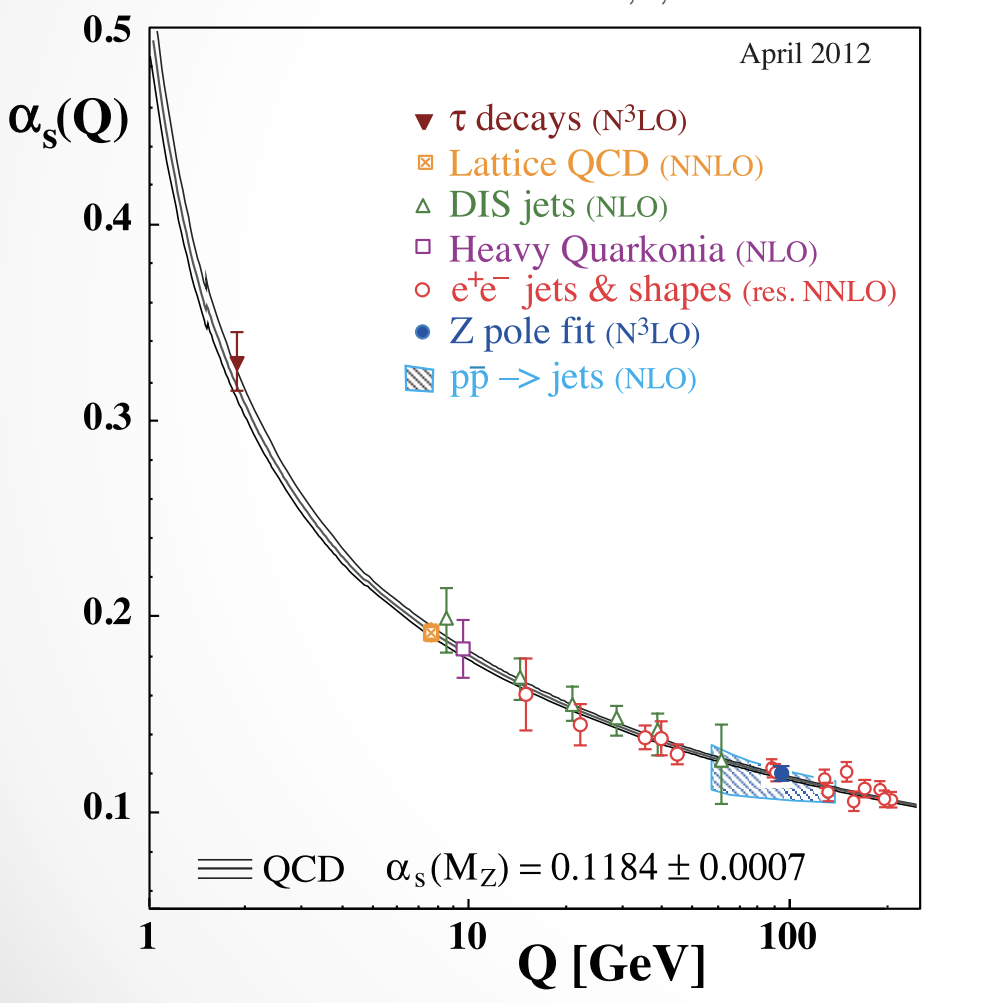
\includegraphics[width=0.6\linewidth]{sm_qcd_coupling}
\caption{Measured values of the strong coupling constant $\alpha_s$ and its predicted values across a range of energies}
\label{fig:sm_qcd_coupling}
\end{figure}\cite{sm-review-2014}

\subsubsection{Asymptotic freedom}

At very high energies, at or above the $GeV$ scale, the strong coupling constant becomes small.
As a result, QCD calculations in this regime are \textit{perturbative},
meaning they can be approximated by a finite sum of terms expanded in powers of the coupling constant.
This is similar to the way calculations are done in quantum electrodynamics (QED).

Asymptotic freedom means that as energy grows infinite,
quarks and gluons can be treated as completely un-coupled, free particles.
At very high energies, their interactions can be treated as small perturbations about the free theory.
At the LHC, the hard-scattering cross-section of a quark from one proton colliding with a quark from another proton
can be calculated in this perturbative way.
However, the full proton-proton collision cross-section calculation requires a combination of both perturbative and non-perturbative calculations.

\subsubsection{Confinement and Hadronization}

At lower energies, the strong coupling constant grows larger, and the theory can no longer be treated as perturbative.
Because the coupling constant is large,
a finite series expanded in powers of the coupling constant is no longer sufficient to estimate the full predictions.
Instead, higher-order terms grow larger and larger, which means an infinite number of such terms would be needed to make an accurate prediction.

The exact energy scale at which QCD becomes non-perturbative is not known,
but experimental evidence indicates that it occurs below approximately $200~GeV$.

Confinement is a consequence of the large coupling constant at low energies.
Since quarks and gluons are strongly coupled, they can no longer exist as free states.
Instead, they can only exist as color-neutral bound states, called hadrons.

In a collision event, when a quark is generated in the final state,
the strong force between the quark and other quarks in the event remains constant as distance between them increases.
Equivalently, the potential energy between quarks increases with distance.
Eventually it becomes energetically favorable for new quarks to be created from the vacuum,
with the correct color charge to neutralize the color charge of the escaping quark.
These new particles become bound together in color-neutral free states.
This process is known as hadronization.

Hadronization, along with parton showering, is responsible for the emergence of jets from LHC collisions.
Rather than observing the quarks and gluons produced in the collision,
the detector can only observe the spray of hadrons that result.
Jets will be discussed in detail in chapter~\ref{ch:jets}.

Confinement has not been rigorously proven from a theoretical standpoint.
However, the existence of color confinement is consistent with empirical evidence.

\subsection{Parton distribution functions}\label{subsec:qcd_pdfs}

The QCD Lagrangian describes how individual quarks and gluons behave.
But the LHC collides protons, not individual quarks.
Protons consist of three valence quarks: two up quarks and one down quark.
But they also consist of a "sea" of quarks and antiquarks, as well as gluons.
When calculating collision cross-sections for the LHC, this internal structure of the protons must be taken into account.

Parton distribution functions (PDFs) model the internal structure of the proton.
They are expressed as probability distributions over momentum fraction $x$, normalized to the number of partons.
The momentum fraction $x$, is the proportion of the proton momentum carried by the individual parton.
PDFs are conditional on $Q^2$, the squared energy scale.
Separate PDFs are calculated for gluons and for each quark flavor.

Examples of PDFs for different quark flavors, as well as for gluons, can be seen in figure~\ref{fig:sm_pdfs}.

\begin{figure}[!ht]
    \centering
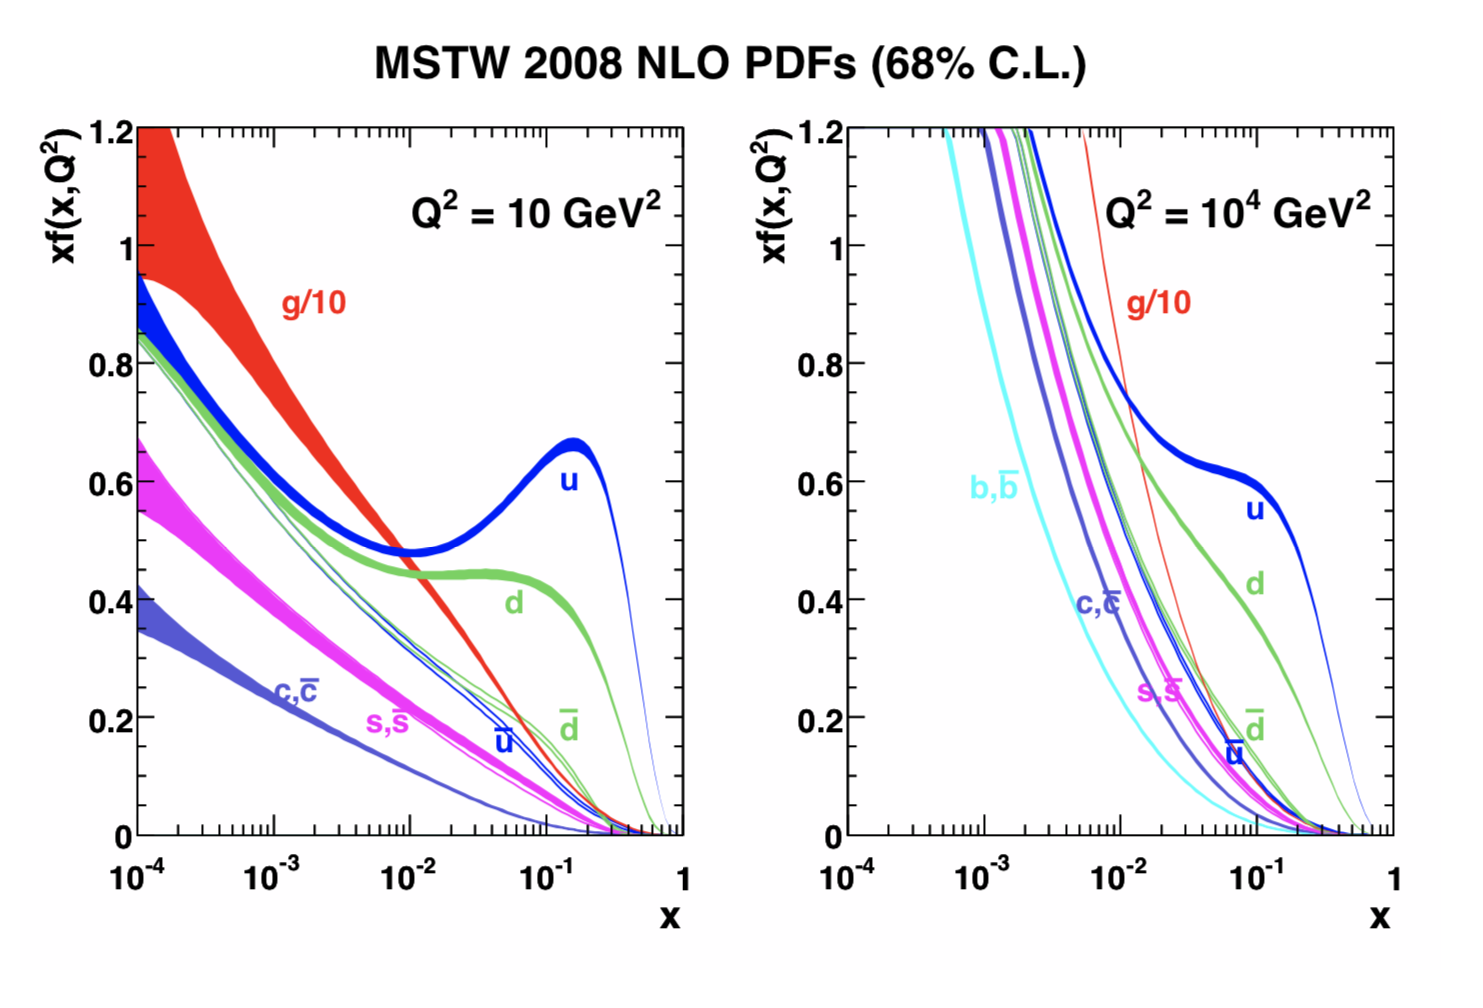
\includegraphics[width=0.6\linewidth]{sm_pdfs}
\caption{Parton distribution functions for the proton, calculated at NLO for two different energy scales.}
\label{fig:sm_pdfs}
\end{figure}\cite{sm-pdf-2009}

When calculating LHC cross-sections, the hard-scattering cross-section for different types of partons
must be convolved with the PDFs for each parton.
The proton-proton cross-sections are thus an average of partonic cross-sections, weighted by the PDFs for those partons.

The factorization theorem of QCD allows for the non-perturbative PDF calculations to be carried out independently from
the perturbative hard scattering cross sections, and then combined.

\section{Limitations}\label{sec:sm_limits}

Experimental tests of the Standard Model to date have shown no significant deviations from its predictions,
across a very wide range of physical processes and energy scales.
However, it is quite clear that the Standard Model is not a complete theory of nature.
For one, it makes no attempt to account for gravitational interactions.
But there are many other problems and questions that it leaves unanswered.

\subsection{Fine tuning and the Higgs mass}\label{subsec:sm_hierarchy}

The Higgs field, which is responsible for the mass of all fundamental fermions and the massive electroweak gauge bosons,
was confirmed by the discovery of $125~GeV$ Higgs boson by ATLAS and CMS in 2012.
The fact that the Higgs mass should be so small is an unsolved mystery of particle physics.

When performing QFT calculations, there often arise terms in the perturbation expansion that are formally infinite.
A procedure known as renormalization is used in order to tame these divergences.
One method of renormalization involves cutting off the divergent integrals at some scale, $\Lambda$,
then canceling the infinities by redefining some of the free parameters of the theories.

When calculating the physical mass-squared of the Higgs, there are some terms in the series which are proportional to the square of the cutoff scale.
The cutoff scale is considered to be some very large energy scale, usually the Planck energy $10^{19}~GeV$.
As a result, an infinite sum of positive and negative terms with absolute values on the order of $10^{38}~GeV^2$ must cancel out
to yield physical Higgs mass-squared, which is on the order of $10^4~GeV^2$.
This kind of cancellation is philosophically unsatisfying, because it seems to be an unreasonable amount of fine-tuning.

The fine-tuning is closely related to the so-called "hierarchy problem".
Why is gravity so much weaker than the other fundamental forces?
That is, why do we observe $G_F \gg G_N$?
Since $G_F \propto 1/{M_W^2}$, and $G_N \propto 1/\Lambda_{Pl}^2$ and because $M_W$ is proportional to the Higgs vev,
the Higgs-mass fine-tuning and the hierarchy problem are really the same thing.

A possible way to avoid fine tuning and the hierarchy problem comes from Supersymmetry, which will be covered in~\ref{ch:susy}

\subsection{Grand unification}\label{subsec:sm_unification}

The symmetry groups and representations of the Standard Model have great explanatory power,
but they are, at heart, axiomatic rather than derived.
The Standard Model contains a large number of free parameters, the values of which are not explained by the model, but must be measured by experiment.

It's possible that a simpler model could be found, one which embeds the baroque structure of the Standard Model in a
much simpler set of symmetry groups and representations.
Such an idea is known as \textit{Grand Unification}.

A Grand Unified Theory (GUT) would predict relationships between some of the free parameters of the Standard Model,
resulting in a simpler and more elegant theory.
This would be analogous to electroweak unification, which explains the relations between $W$ and $Z$ boson masses,
as well as their couplings.
As a result, the theory has only three free parameters, and the rest can be determined once those are known.

The GUT would explain all particle interactions with a single symmetry group.
This symmetry would be broken below some energy scale to the $SU(3)_C \times SU(2)_L \times U(1)_Y$ symmetry of the Standard Model.
The details of the symmetry breaking process would yield relations between the strong and electroweak coupling constants.

Going a step further, if gravitational interactions could also be incorporated into this single theory,
it would be a so-called "Theory of Everything" (TOE).
A very popular TOE candidate, known as String Theory, relies on the existence of Supersymmetry.

\subsection{Dark Matter}\label{subsec:sm_dark_matter}

The type of matter explained by the Standard Model is known to account for approximately $20\%$ of the matter in the universe.
The remaining $80\%$ exists in the form of dark matter.
The exact explanation for dark matter is not yet known, those many of its properties can be inferred.
It is massive and invisible, and its primary interaction with visible matter is through gravity.

Dark matter is known to be massive, because it interacts gravitationally.
This can be seen in its effect on the rotation curves of galaxies, gravitational lensing of distant galaxies,
and on the anisotropy of the Cosmic Microwave Background Radiation.

Dark matter could possibly be explained by the Standard Model, if it exists in the form of Massive Compact Halo Objects (MACHOs).
This form of dark matter is become less and less favored by experimental measurements over time.

Another likely explanation for dark matter is that it is composed of a new fundamental particle,
one which is not explained by the Standard Model.
Many versions of Supersymmetry, described in~\ref{ch:susy}, provide a viable dark matter candidate.

